\section{Fitting Diffusion Barriers using Neural Network}
\label{Chap:Al/Vac:section:NN}

The computational engine that provided the energetics used to evaluate energy differences and activation barriers before and after vacancy jump in Al 7075 alloy was the implementation of \ac{DFT} together with \acf{CI-NEB} in the \ac{VASP} software with VTST package from Henkelman's group \cite{henkelman2000climbing,henkelman2000improved}.
\ac{CI-NEB} method is used to search reaction pathways. The \acf{NEB} is a general method for finding saddle points and minimum energy paths between known reactant and product atomic configurations. This method works by optimizing a certain number of intermediate images along the reaction path. Each image finds the lowest possible energy while maintaining linear spline spacing to neighboring images. This is done by adding spring forces along the band between images and by projecting out the force component parallel to the band due to the interatomic potential. The \ac{CI-NEB} method modifies the \ac{NEB} method in a way that the highest-energy image is pushed up to the saddle point by trying to maximize its energy along the band and minimize in all other directions. When the algorithm converges, the highest-energy image will be at the exact saddle point, so a smaller number of intermediate images is needed in \ac{CI-NEB} than \ac{NEB}. With this setup, we can use high-throughput calculations to extract forward/backward activation barriers by calculating the energy differences between the image of the highest energy and the initial/final image.


All-electron \ac{PAW} potentials were employed for the elemental constituents with the \ac{GGA} of \ac{PBE} for the exchange-correlation energy functional, $\mu_{xc}$, and the interpolation formula of Vosko et al. \cite{vosko1980accurate}. Using plane-wave cutoff energy of at 450.0 eV, the total energy for all models of initial and final images was converged to $10^{−7}$ eV/cell. The reciprocal space of bulk supercells was sampled with (2x2x2) k-point grids. Each grid was generated using the Monkhorst-Pack scheme \cite{monkhorst1976special}. A (4x4x4) conventional supercell with a single vacancy embedded was used for these calculations. For activation barrier calculations, 5 images between relaxed initial and final images were used. A spring constant was set to 5 $\text{eV}/\angstrom^2$. The force convergence criteria for all models was set to be less than 0.05 $\text{eV}/\angstrom$. The force-based quick-min optimizer was used to make \ac{NEB} calculations stable for high local concentration cases. \cite{sheppard2008optimization}


We calculated lattice constant for Al 7075 alloy, using \acfp{SQS} method \cite{zunger1990special}. A (4x4x4) conventional supercell with 256 atoms was used. The types of 256 atom was chosen to be 244 Al atoms, 7 Mg atoms, and 5 Zn atoms, which is within the concentration range of Al 7075 alloy. The obtained lattice constant is 4.05838 \angstrom, which is roughly the lattice constant (4.041\angstrom) of pure Al considering that Zn and Mg atomic weights are not high. \cite{haas2009calculation}


To sample a larger potential energy landscape, our \ac{NN} model training set contains mainly two different parts, as shown in Fig. \ref{Chap:Al/Vac:fig:atomic_illu}: 1) (4x4x4) randomly generated solid-solution structures with different local concentrations around jump pairs. 2) (2x2x2) randomly generated ordered structures embedded in (4x4x4) pure Al. The first training set is good for simulating vacancy diffusion of a very early stage, during which Al alloy is in the solid-solution state. The second training set is designed to accurately describe the behavior of vacancy moving across/along the boundary between solid-solution Al and ordered phases, and moving inside the ordered phases. The atomic structures of ordered phases are chosen from proposed GP zone structures from \cite{berg2001gp} and low energy ordered $\text{L1}_\text{0}, \text{L1}_\text{2}, \text{L1}_\text{0}^*, \text{W2}, \text{CH}, \text{L1}_\text{2}^*, \text{Z1}$ structures of Au-Fe from \cite{zhuravlev2017phase} with random species perturbation. The atomic  structures were generated using our in-house code KNN2. \cite{Zhang2020KNN2} \textbf{Ordered structure part of the generation code is written by my colleague, Zhucong Xi.}


\begingroup
\begin{figure}[!ht]
  \centering
  \subfigure[]{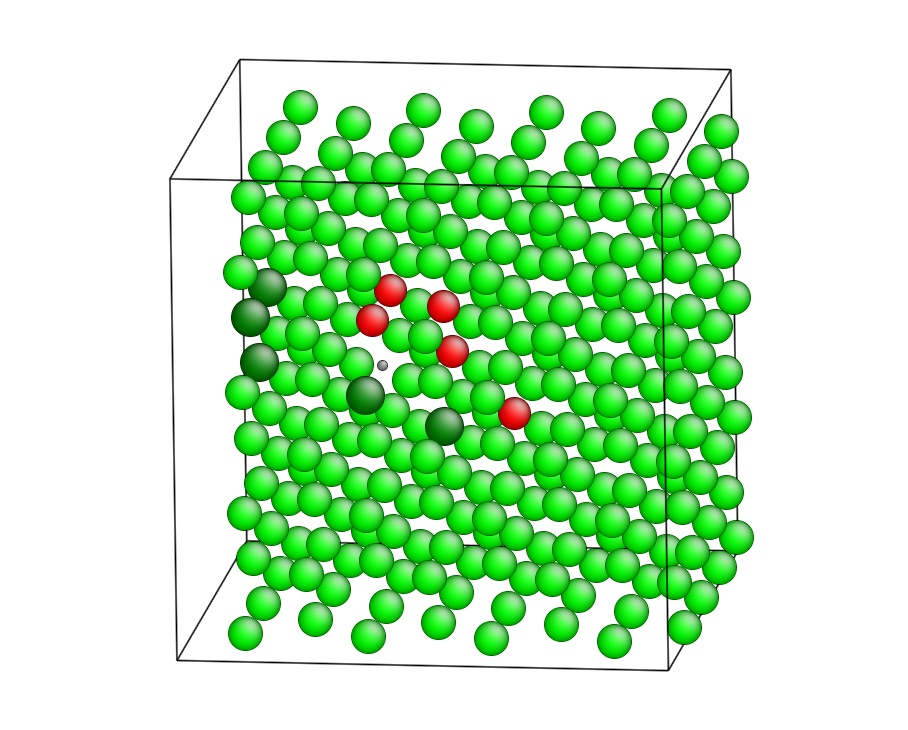
\includegraphics[width=0.49\linewidth]{Chap5/plots/ss_atomic.jpg}}
  \subfigure[]{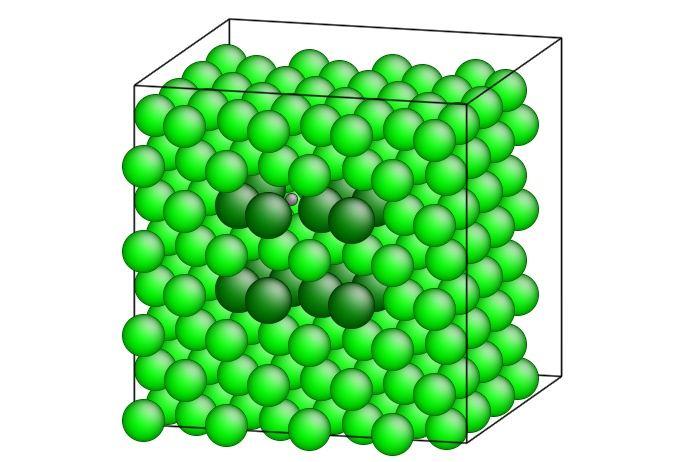
\includegraphics[width=0.49\linewidth]{Chap5/plots/ordered_atomic.jpg}}
\caption[Atomistic pictures of (4x4x4) supercells containing 256 atoms.]{Atomistic pictures of (4x4x4) supercells containing 256 atoms. (a) One typical (4x4x4) randomly generated solid-solution structure. (b) One typical (2x2x2) randomly generated ordered structures embedded in (4x4x4) pure Al. Light green, dark green, and red atoms are Al, Mg, and Zn, respectively. The small gray atom represents the location of vacancy.}
\label{Chap:Al/Vac:fig:atomic_illu}
\end{figure}
\endgroup


Many different machine learning/deep learning models are widely used, each one suitable for a different kind of problem. \cite{bartok2010gaussian,behler2011atom,szlachta2014accuracy,artrith2016implementation,mehta2014exact,artrith2017efficient} For our particular problem, the feed-forward Artificial Neural Network (ANN) is chosen, as it provides a general frame to map non-linear input (atomic species of neighboring environment) to a continuous regressor (diffusion barriers). It is well known that a sufficiently large number of hidden neurons can approximate any continuous multivariate function. \cite{hornik1989multilayer} This property gives us the most expandability of this framework when the system needs to go even further complicated in terms of the number of species considered. 


The output layer of our \ac{NN} model predicts diffusion barriers in a 1-D continuous space. The input layer was chosen to be 27 discrete numbers representing atom species based on Ising model, as shown in Table. \ref{Chap:Al/Vac:tab:mapping}. Among the 27 numbers, the first one indicates the type of atom that will be swap with the vacancy. The rest 26 (each atom has 12 + 6 = 18 $\text{2}^{nd}$ nearest neighbors. And both of them share 10 in common.) atoms represents the neighboring atoms of the jump pair up to their $\text{2}^{nd}$ nearest neighbors, as shown in Fig. \ref{Chap:Al/Vac:fig:2nn}. The rest 26 numbers are arranged in their geographical order (ascending in X, Y, and Z accordingly), so their position will always respond to the same input neuron in the \ac{NN} architecture. Besides, this cluster of 26 neighboring atoms also has 2-fold symmetry  ($R_{2 fold} = \begin{bmatrix} 1 & 0 & 0 \\0 & -1 & 0 \\0 & 0 & -1 \\\end{bmatrix}$), mirror symmetry along Y-Z plane ($R_{x mirror} = \begin{bmatrix} -1 & 0 & 0 \\0 & 1 & 0 \\0 & 0 & 1 \\\end{bmatrix}$), and mirror symmetry along the X-Y plane($R_{z mirror} = \begin{bmatrix} 1 & 0 & 0 \\0 & 1 & 0 \\0 & 0 & -1 \\\end{bmatrix}$). Therefore, for one jumping event, the diffusion barrier is taken as the average of the four symmetric configurations of the 26 neighboring atoms to have a rotation-invariant prediction. Details of this method is described in Algorithm. \ref{algo:encode}. By using several layers of hidden neurons between 27 input species and 1 output diffusion barrier, the contribution distribution to final output, diffusion barrier, of pair-wise and triple-wise interactions can be learned.

\begin{figure}[!htb]
  \centering
  \begin{minipage}{.7\linewidth}
    \begin{algorithm}[H]
      \caption{Jumping Pair Encoding Algorithm}\label{algo:encode}
      \begin{algorithmic}[1]
        \State set a reference matrix as a 3x3 identity matrix, $m_0$ = $$\begin{bmatrix} 1 & 0 & 0 \\0 & 1 & 0 \\0 & 0 & 1 \\\end{bmatrix}\quad$$.
        
        \State determine the jumping direction $v_0 = r_{atom} - r_{vac}$, where $r$ is the coordinates of atom/vacancy. Noting that in the practice, atoms may need to be wrapped according to periodic boundary conditions.
        \State determine all the 26 neighboring atoms of the ghost atom at the vacancy site and the jumping atom within the $2^{nd}$ nearest neighbor distance cutoff.
        \State randomly pick one $2^{nd}$ nearest neighbor atom with coordinates $r_1$ of the vacancy atom, and calculate $v_1 = r_{1} - r_{vac}$.
        \State calculate $v_2 = v_0 \cdot v_1$.
        \State concatenate matrix $m_1$ = $\begin{bmatrix} v_0 \\v_1 \\v_2 \\\end{bmatrix}$.
        
        \State calculate rotation matrix $R$ for projecting $m_1$ to the reference coordinate $m_0$. 
        \State rotate coordinates of all the 26 atoms by applying the rotation matrix $R$ to project all the atoms need to encode along the same reference directions. The new coordinates denotes as $r'$. 
        \State encode atoms based on the preset mapping of type, and ascending order in X, Y, and Z coordinates accordingly.
        \State apply for the three rotational matrices, 
        $R_{2 fold} = \begin{bmatrix} 1 & 0 & 0 \\
                                      0 & -1 & 0 \\
                                      0 & 0 & -1 \\
        \end{bmatrix}\quad$
        $R_{x mirror} = \begin{bmatrix} -1 & 0 & 0 \\
                                         0 & 1 & 0 \\
                                         0 & 0 & 1 \\
        \end{bmatrix}\quad$
        $R_{z mirror} = \begin{bmatrix} 1 & 0 & 0 \\
                                        0 & 1 & 0 \\
                                        0 & 0 & -1 \\
        \end{bmatrix}\quad$
        , to the coordinates $r'$ and encode them use the same method mentioned above.
        
      \end{algorithmic}
    \end{algorithm}
  \end{minipage}
\end{figure}


\begin{table}[!htbp]
\centering
\caption[Atom species encoding map for the \acf{NN} input layer.]{Atom species encoding map for the \acf{NN} input layer. Here, ``Vac'' represents vacancies.}
\label{Chap:Al/Vac:tab:mapping}
\begin{tabular}{cc}
\\
\hline
\hline
Species & Encoding  \\ \hline
Al & 1.0 \\
Mg & 2.0 \\
Zn & 3.0 \\
Vac & 4.0 \\
\hline
\hline
\end{tabular}
\end{table}


\begingroup
\begin{figure}[!ht]
  \centering
  \subfigure{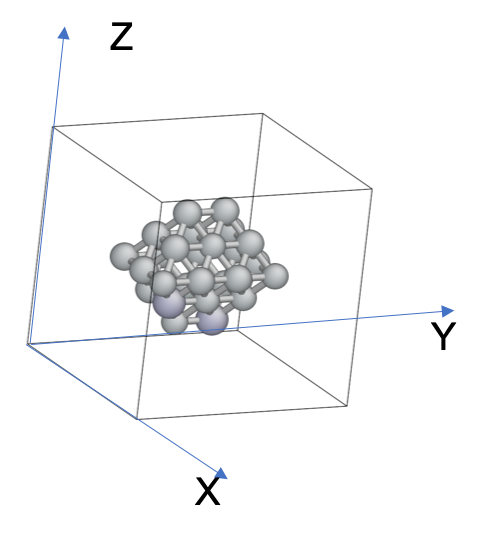
\includegraphics[width=0.5\linewidth]{Chap5/plots/2nn.png}}
\caption[Illustration of atomic structures of the $\text{2}^{nd}$ nearest neighbors surrounding the jumping pairs.]{Illustration of atomic structures of the $\text{2}^{nd}$ nearest neighbors surrounding the jumping pairs. The 26 neighboring atoms have 2-fold symmetry, mirror symmetry along Y-Z plane, and mirror symmetry along the X-Y plane.}
\label{Chap:Al/Vac:fig:2nn}
\end{figure}
\endgroup


We implemented the \ac{NN} model using Google's TensorFlow \cite{abadi2016tensorflow} with Keras \cite{chollet2015keras}. TensorFlow is an open source numerical computation framework using data flow graphs with the ability of deriving gradients automatically. Keras is a high-level neural networks API, written in Python and capable of running on top of TensorFlow. The optimized neural network structures was tuned by Talos \cite{Autonomio2019Talos}. The Adam optimizer \cite{kingma2014adam} was used for optimizing weights in the neural network. Xavier uniform initializer \cite{glorot2010understanding} was used to generate the random weights and biases so as to break the symmetry of weighting parameters. The activation functions were chosen to be \acf{ReLu} for all the hidden layers. The activation function for the output layer is chosen to be linear to predict diffusion barriers on a continuous scale. Normalization method was also been tested but not helpful on accuracy, as diffusion barriers follow very good normal distribution.  The optimized \ac{NN} architecture can be found in Table. \ref{Chap:Al/Vac:tab:NN}. Large neural nets trained on relatively small datasets can overfit the training data. Generalization will have low performance on accuracy of new data due to overfitting. Dropout is a regularization method to prevent overfitting. This introduce a new hyperparameter, dropout probability, as listed in Table. \ref{Chap:Al/Vac:tab:NN}. Though more complicated \acf{RBM} and many other generative stochastic artificial neural networks can be used as a function approximator, their complexity will slow down the \ac{KMC} iterations significantly.


\begin{table}[!htbp]
\centering
\caption[Neural network architecture with activation functions and dropout probability of each layer.]{Neural network architecture with activation functions and dropout probability of each layer.}
\label{Chap:Al/Vac:tab:NN}
\begin{tabular}{cccc}
\\
\hline
\hline
Layer & Shape  & Activation  & Dropout Probability\\ 
\hline
Dense & 256    & ReLu       & 0.1                 \\
Dense & 256    & ReLu       & 0.2                 \\
Dense & 128    & ReLu       & 0.0                 \\
Dense & 64     & ReLu       & 0.05                \\
Dense & 64     & ReLu       & 0.0                 \\
Dense & 16     & ReLu       & 0.0                 \\
Dense & 1      & Linear     & N.A.                \\ 
\hline
\hline
\end{tabular}
\end{table}


To train the \ac{NN}, two different loss functions are used. The former one is the common \acf{MSE} via:
\begin{subequations}
\begin{align}
MSE = \frac{1}{N}\sum_{i=1}^{N}({E_a}_{i}^{DFT} - {E_a}_{i}^{NN})^2
\label{Chap:Al/Vac:eq:MSE}
\end{align}
\end{subequations}
where $N$ is the number of input datas, which can be trained in batch or mini-batch, ${E_a}_i^{DFT}$ is the diffusion barrier of $i^{\text{th}}$ data from \ac{DFT} calculation, and ${E_a}_{i}^{NN}$ is from \ac{NN} prediction. As shown in Fig. \ref{Chap:Al/Vac:fig:fitting_all}, the model reached a \ac{RMSE} of 0.04313 eV/atom for all the data points. The latter one is a customized loss function, via:
\begin{subequations}
\begin{align}
Loss = \frac{1}{N}\sum_{i=1}^{N}{(1.0 + \alpha (1.5 - {E_a}_{i}^{DFT})({E_a}_{i}^{DFT} - {E_a}_{i}^{NN})^2)}
\label{Chap:Al/Vac:eq:custLoss}
\end{align}
\end{subequations}
where $\alpha$ is a tunable knob. A larger $\alpha$ value will weigh more on diffusion barriers that are small. In this way, we are able to fit low-energy barriers more accurately, as they are the critical rate-determining steps in a \ac{KMC} simulation. Using this custom loss function, the model reached a \ac{RMSE} of 0.03785 eV/atom for all the data points. Noting that the model trained using the latter loss function is slightly more accurate than the former method because more data points are located far away from 1.5 eV. As we expected, low-energy barriers are predicted with higher accuracy, which can be seen from Fig. \ref{Chap:Al/Vac:fig:fitting_all_weighted}.


\begingroup
\begin{figure}[!ht]
  \centering
  \subfigure[]{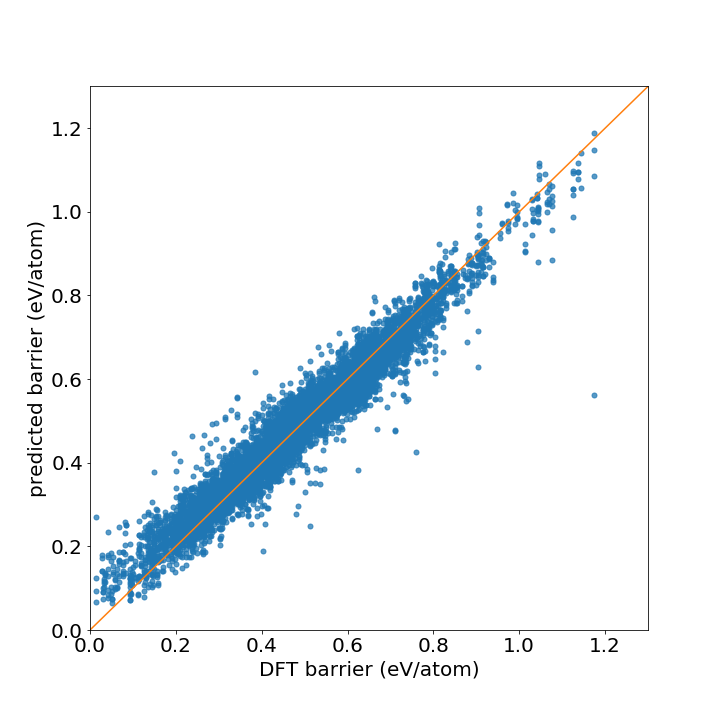
\includegraphics[width=0.49\linewidth]{Chap5/plots/total.png}}
  \subfigure[]{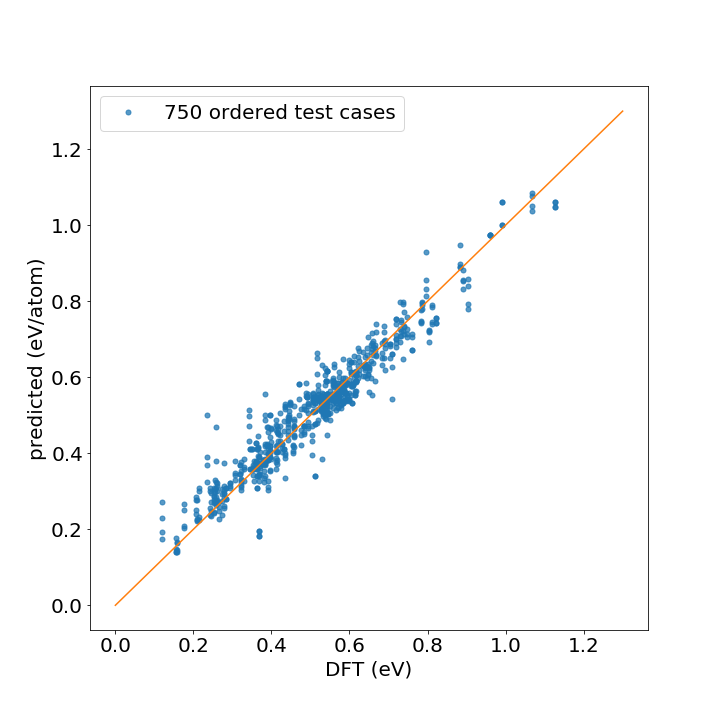
\includegraphics[width=0.49\linewidth]{Chap5/plots/fit_ordered.png}}
\caption[Predictions accuracy of diffusion barriers from neural network surrogate model, compared with DFT calculated results.]{Predictions accuracy of diffusion barriers from neural network surrogate model, compared with DFT calculated results. The orange solid line indicates perfect fitting. Each blue solid dot represents one data point. (a) predictions of all the barriers. (b) predictions of ternary ordered structures.}
\label{Chap:Al/Vac:fig:fitting_all}
\end{figure}
\endgroup

\begingroup
\begin{figure}[!ht]
  \centering
  \subfigure[]{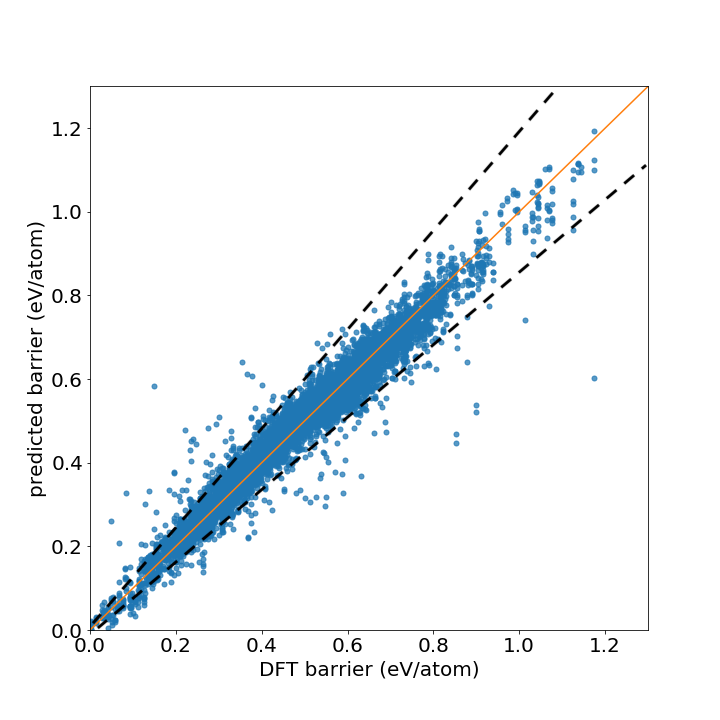
\includegraphics[width=0.49\linewidth]{Chap5/plots/total_weighted.png}}
  \subfigure[]{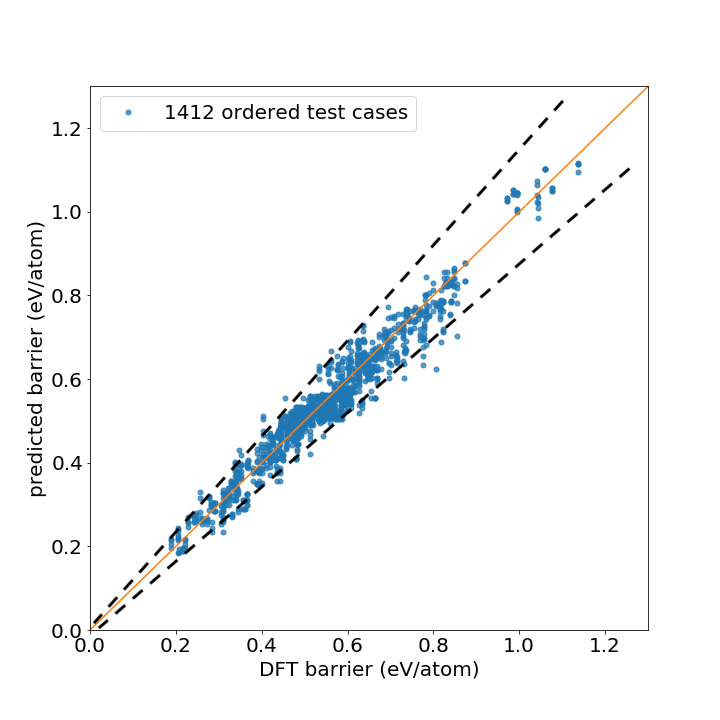
\includegraphics[width=0.49\linewidth]{Chap5/plots/fit_ordered_weighted.png}}
\caption[Predictions accuracy of diffusion barriers from neural network model using custom loss function, compared with DFT calculated results.]{Predictions accuracy of diffusion barriers from neural network model using custom loss function, compared with DFT calculated results. During model training, Equation. \ref{Chap:Al/Vac:eq:custLoss} was used to weigh more on low-energy barriers. The orange solid line indicates perfect fitting. Each blue solid dot represents one data point. The black dashed lines illustrate the confinement introduced by custom loss function with emphasis on low-energy-barrier data points. (a) predictions of all the barriers. (b) predictions of ternary ordered structures.}
\label{Chap:Al/Vac:fig:fitting_all_weighted}
\end{figure}
\endgroup